\documentclass[11pt,english]{article}
\usepackage{ae,aecompl}
\usepackage{helvet}
\usepackage[T1]{fontenc}
\usepackage[sort&compress,super]{natbib}
\citestyle{naturemag}
\usepackage{amssymb,amsmath,amsthm}
%\usepackage[nolists]{endfloat}
\usepackage{graphicx}
\usepackage[pdfborder={0 0 0}]{hyperref}
\usepackage{chngpage}
\usepackage{pdflscape}
\usepackage{epstopdf}
\usepackage{fullpage}
\usepackage{setspace}
\usepackage{booktabs}
\usepackage{subfigure}
\usepackage[small,compact]{titlesec}
\usepackage{rotate}

\usepackage{xr-hyper}
\usepackage{hyperref}
\externaldocument{Stacking_APPENDIX}


\newcommand{\noun}[1]{\textsc{#1}}

\providecommand{\tabularnewline}{\\}

\theoremstyle{plain} \newtheorem{claim}{Claim}
\theoremstyle{plain} \newtheorem{prop}{Proposition}
\theoremstyle{plain} \newtheorem{hypo}{Hypothesis}

\bibpunct{}{}{,}{s}{}{}

\begin{document} 

\title{Jointly Modeling the Adoption, Consumption, and Exclusive Use of Clean Cooking Fuels in Rural India\thanks{We thank the Council on Energy, Environment and Water (CEEW) for their collaboration on both rounds of the ACCESS survey, funded by the Shakti Sustainable Energy Foundation and the National University of Singapore. We thank Micha\"{e}l Aklin and Namrata Chindarkar for their contributions to the ACCESS survey. If this article is published, a full replication archive with all data and code will be made available.}}

\author{Carlos F. Gould\footnote{Indicates that these authors are co-first authors. CFG led the writing and XH led the statistical analysis.}\\Columbia University Mailman School of Public Health\and  Xiaoxue Hou$^\dagger$\\Johns Hopkins SAIS \and Jennifer Richmond\\University of Maryland \and Anjali Sharma\\University of Maryland \and Johannes Urpelainen\footnote{Corresponding author. Address: Rome Building, 4th Floor. 1619 Massachusetts Avenue, NW. Washington, DC 20036, USA. Tel: +1-734-757-0161. Email: JohannesU@jhu.edu.}\\Johns Hopkins SAIS}

\maketitle

\begin{abstract}
Solid fuel combustion is a major cause of household air pollution, a leading environmental health risk factor globally. In India, over 750 million people continue to rely on firewood and other solid fuels for their daily cooking. Here we explore the drivers of adoption, consumption, and exclusive use of liquefied petroleum gas (LPG), India's dominant clean cooking fuel. Using ACCESS, a panel dataset of over 8,500 rural households from six Indian states surveyed in 2015 and 2018, we document impressive strides in LPG ownership, partially due to \emph{Pradhan Mantri Ujjwala Yojana}, India's flagship clean cooking policy. We further demonstrate that the drivers of initial LPG adoption also apply to consumption and exclusive use. While fuel stacking -- most households continue to use solid fuels and LPG jointly -- is a challenge, improved rural incomes and education result in the exclusive use of clean cooking fuels. However, we find that PMUY beneficiaries consume 27 kilograms of LPG less than general customers on average per year, even after accounting for baseline socio-economic differences and years of using LPG. Our findings suggest that additional strategies to accelerate the transition to exclusive LPG use among the 80 million households acquiring LPG through PMUY, such as enhanced cylinder distribution points to reduce access costs, are necessary to yield the full benefits of the Government of India's investments in cleaner cooking.
\end{abstract}

\textbf{Keywords}: clean cooking; energy access; survey research; India; PMUY; energy policy

\clearpage

\doublespacing

Widespread solid fuel combustion to meet daily household cooking and heating needs has profound global impacts on health\citep{Stanawayetal2018,HEI2018}, climate \citep{Bondetal2004}, the environment\citep{Bailisetal2015}, and women's empowerment\citep{Rosenthaletal2018}. Roughly 2.8 billion people worldwide\citep{Bonjouretal2013}, and more than 750 million people in India alone\citep{Balakrishnanetal2019}, rely on inefficiently burning solid fuels like wood, dung, charcoal, or agricultural residues to meet their daily household energy needs, resulting in high levels of household air pollution (HAP). An estimated 480,000 (95\% confidence interval, 390,000--580,000) premature deaths in India were attributable to HAP exposure alone in 2017\citep{Balakrishnanetal2019}, with potentially more than 100,000 premature deaths from ambient air pollution attributable to contributions from residential emissions\citep{Chowdhuryetal2019a}. Clean cooking fuels promise substantial benefits from reduced HAP exposure, solid fuel collection, and drudgery. Yet, the adoption and sustained use of clean cooking fuels remains limited across much of the world's resource-poor rural communities; even rarer still is the cessation of cooking with solid fuels that is needed to obtain clean kitchens and healthy homes\citep{Popeetal2017}.

India is in the midst of a nationwide transition to cleaner cooking -- a costly effort that promises substantial benefits -- but patterns of cooking fuel use in households after the adoption of liquefied petroleum gas (LPG) stove remain poorly described. While LPG is a popular cooking fuel in rural India\citep{GouldUrpelainen2018}, lessons from around the world show that households adopting a clean cooking fuel commonly continue to use their traditional stoves and fuels -- a practice termed fuel stacking -- rather than fully replace their previous cooking practices\citep{RuizMercadoMasera2015,Pillarisettietal2014}. Partial transitions to clean cooking are unlikely to lower air pollution levels enough to significantly reduce health risk \citep{JohnsonChiang2015}. Therefore, understanding the determinants of clean cooking fuel adoption and use, as well as the reasons for fuel stacking, can inform measures that facilitate increases in clean fuel use and the reduction of solid fuel use so Indian households can reap the full rewards of clean cooking. 

Previous studies and reviews have pointed to the roles of individual (perceptions, preferences), household (demographics, socio-economic status), local environmental (climate), and contextual (fuel prices and availability, policies) characteristics in determining the adoption and use of clean cooking fuels\citep{MullerYan2018,Quinnetal2018,Puzzoloetal2016,LewisPattanayak2012}. Still, the extent to which households use a clean cooking fuel after adoption has received comparatively little attention despite the inherently successive process of technology adoption and use. Study of cooking fuel choice has been limited by three common traits. First, most studies lack longitudinal data that are unable to capture within-household fuel transitions over time and limit analytic approaches. Second, for many years, surveys have only asked about a household's primary cooking fuel. While this trend has changed in recent years, much of the available empirical analysis on cooking fuel choice has been unable to model fuel stacking. Third, long lags between data collection and availability has diminished the ability to analyze current fuel choices in a policy-relevant time frame, in particular when utilizing regionally- or nationally-representative surveys. This latency shortcoming is particularly relevant when household fuel choices are affected by ongoing policies that may be responsive to new evidence, such as those ongoing currently in India. 

There have been a few recent studies addressing these limitations on which we build. A recent study leveraging a cohort from three provinces in China from 1995 to 2016 shows that the determinants of clean fuel adoption and the determinants of the suspension solid fuel use differ somewhat\citep{Carteretal2019}. Higher household incomes, younger household heads, and smaller household sizes were associated with clean fuel adoption, whereas younger age and being widowed was associated with solid fuel suspension and younger age, greater education, and poor self-reported health status was associated with earlier solid fuel suspension. Two recent studies in Tanzania\citep{ChoumertNkoloetal2019} and Ethiopia\citep{Alemetal2016} used three rounds of panel survey data to assess the socio-economic determinants of fuel stacking behavior, finding household expenditures, education, and fuel prices to be associated with fuel choice. However, neither household models within-household fuel switching and both include kerosene as a ``clean" cooking fuel, despite current evidence that burning kerosene emits high air pollution leading to substantial health risk\citep{Lametal2012}. In addition, a companion study to our own assesses the determinants of fuel stacking category among LPG-owners in 2018 and models within-household shifts in the use of both LPG and solid fuels among rural LPG-owners in India from 2015 to 2018\citep{Tripathietal2020}. PMUY beneficiaries had lower odds of using LPG as their exclusive or even primary cooking fuel as compared to general consumers. Years with LPG and household wealth were associated with upward movement in LPG use category. These studies have advanced our understanding of fuel stacking and emphasize the need to model the adoption of clean cooking fuels alongside the cessation of solid fuel use to identify energy policies that benefit health, economy, and environment. 

% Two recent studies in India use multiple rounds of the National Sample Survey to assess the determinants of multiple cooking fuel use. The first study shows a strong association between increasing expenditures and clean cooking fuel use using the 50th round (1993-1994), the 61st round (2004-2005), and the 66th round (2009-2010), but the study lacks repeated measurements and therefore cannot model within-household changes over time\citep{SwarupRao2015}. The second study creates a synthetic panel of about 100,000 households matched on their State, urban/rural, and caste from the 55th round (1999-2000) and the 68th round (2011-2012) to assess the extent to which LPG has offset firewood use. However, this study does not study the determinants of fuel switching or fuel stacking\citep{Singhetal2017}. 

This study addresses three principal questions: 1) What factors are linked to a household's probability of adopting LPG? 2) If a household does adopt LPG, what determines whether or not a household continues solid fuel use and which fuel (LPG or a solid fuel) is dominant? and 3) What factors predict overall LPG consumption if a household does adopt LPG? 

We use a comprehensive energy access survey administered in more than eight thousand rural households across six energy-poor Indian states in 2014-2015 and then again in 2018. We find that the extent of LPG use has increased substantially since 2015, but that the majority of households continue to use solid fuels for cooking. More than 80\% of study households rely on solid fuels to meet some of their cooking needs in 2018. Still, exclusive clean cooking fuel use has increased from less than 5\% to nearly 17\% in just three years. We find that households with greater monthly expenditures, more educated household heads, and those that belong to the general caste category use cleaner cooking fuel stacks -- those that are less reliant on solid fuels. To model LPG use patterns, we leverage our panel data structure to jointly model LPG adoption and use in a two-stage hurdle model. We find that the same determinants of LPG adoption -- expenditures and education -- also explain LPG consumption. Still, we find that PMUY beneficiaries are predicted to consume about 35\% less LPG than general customers after accounting for baseline socio-economic and demographic differences across households and the years of experience using LPG. 

These findings provide insights for future policies promoting clean cooking fuel use in India. India's advancements in LPG adoption through innovative government programs are worthy of praise. However, policies targeting the cessation or reduction of solid fuel use may be needed to improve health through reductions in HAP exposure. Second, our findings that the same factors determine both LPG adoption and use suggest that initiatives that lower the costs of LPG, including cylinder refill prices and accessibility, may accelerate cleaner stacking practices. Finally, the result that education is also a robust predictor of LPG adoption and use suggests that awareness efforts should be a feature of government programs.


\section*{Transitions to Clean Cooking Fuels in India}

LPG has historically been too expensive or unreliably accessible for use in most rural households in India and around the world\citep{Kumar2016,Quinnetal2018}. In response, the Government of India and the country's largest Oil Marketing Companies (OMCs) have launched a series of state and national policies to increase clean cooking among the country's poorest households over the last ten years.

The ambitious Pradhan Mantri Ujjwala Yojana (PMUY) was launched in 2016 and plans to provide 80 million LPG connections -- the ability to purchase LPG cylinder refills from the national market -- to below-poverty-line households by 2020 (increased from its original goal of 50 million connections)\citep{MoPNG2018}. PMUY leads India's national LPG program and has received substantial international attention. However, the Government of India has been facilitating the use of LPG since the late 2000s by improving accessibility and lowering costs. The Rajiv Gandhi Grameen LPG Vitrak (RGGLV) scheme was launched in 2009 to increase LPG distribution in remote areas by increasing LPG coverage and providing below-poverty-line families a one-time grant for new LPG connections. Later in 2016, rural LPG distribution was further improved by increasing the reliability of cylinder refill supply and implementing direct home  refill deliveries. In 2015, the Direct Benefit Transfer for LPG (DBTL), or PAHAL, developed a system to directly deposit the difference between the market and subsidized cost of cylinder refills into participants' bank accounts, facilitating a flexible and more efficient subsidy transfer system\citep{Jainetal2018}. The next year, the ``Give it Up" program enrolled more than 10 million LPG consumers to voluntarily discontinue their subsidy and transfer it to below-poverty-line households. Through PMUY, the Government of India then allocated more than 1 billion USD to provide assistance of 1,600 Indian Rupees (INR) for each connection to subsidize the LPG cylinder deposit and regulator and installation charges. Households then purchase a double-burner LPG stove (1000 INR) and their first LPG cylinder (500 INR) with optional loan assistance. PMUY has also been successful at expanding the network of LPG distributors in rural India. After expansions of eligible beneficiaries, 80 million new LPG connections have been established since 2016\citep{MOPNG2019}. 

Fig. \ref{lpgtransition} highlights how the penetration of LPG into rural areas has increased, especially in historically energy-poor states of India such as Uttar Pradesh and Bihar where LPG ownership has more than doubled in the last three years. Between 1993 and 2012, the share of rural households using LPG as their primary cooking fuel increased from approximately 2\% to 15\% as solid fuels remained the primary source of household energy for more than three-quarters of rural Indians\citep{NationalSampleSurvey2015}. The impact of PMUY and other LPG programs is clear: access to LPG in rural India has increased at an unprecedented rate since 2015. Now, more than an estimated 85\% of Indian households have an LPG stove and cylinder\citep{MOPNG2019}, though recent data collection as a part of the 76th round of the National Sample Survey in late 2018 suggests actual household use may be lower\citep{MOSPI2019}.

 
\begin{figure}[h!]
\centering
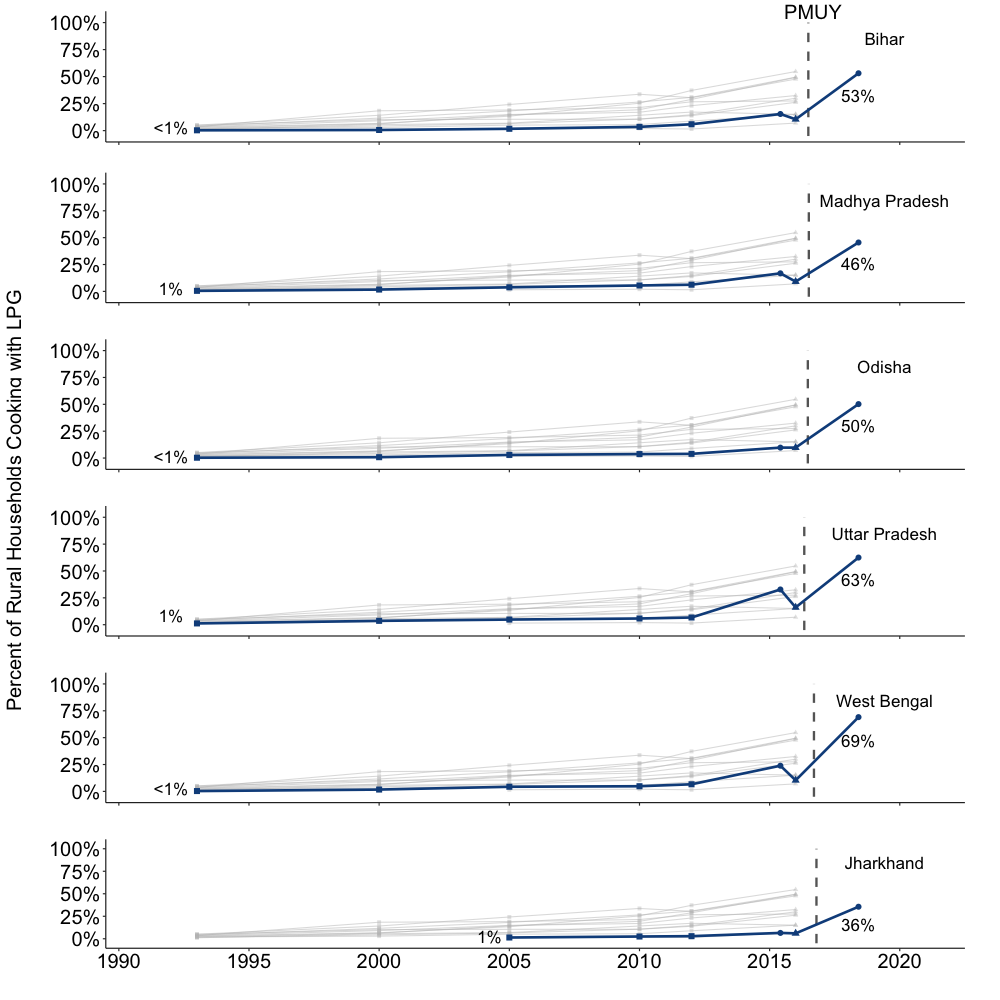
\includegraphics[scale=0.46]{Figures/StateLPGTransition_Facet_Rural.png}
\caption{\textbf{LPG use as a cooking fuel is increasing across rural India and in historically energy-poor study states.} Blue lines highlight the increases in LPG use as a cooking fuel in rural households in study states, while grey lines show the rest of states in India over the same time period. We combined several freely-available sources to provide historical state-level estimates of LPG use in rural Indian households: (i) the National Sample Survey provided estimates in 1992-1993, 1999-2000, 2004-2005, 2009-2010, and 2011-2012; (ii) the India National Family Health Survey provided estimates in 2015-2016; and (iii) ACCESS I and II provided study state estimates in 2015-2016 and 2017-2018.}
\label{lpgtransition}
\end{figure}

Despite great advances in LPG stove ownership across the nation, relatively little is known about the extent to which LPG is displacing the use of solid fuels for cooking. Data on new LPG connections -- a marker of the ability to use LPG stoves -- are regularly updated; however, information detailing LPG cylinder refills consumed by PMUY beneficiaries remain limited\citep{Dabadgeetal2018,MoPNG2019b}. Based on available aggregate data, one-quarter of households are estimated to purchase five or more cylinder refills but approximately 20\% do not return for a single refill in their first year of LPG ownership\citep{Karetal2019a,TheTimesIndia2019}. In a study of one rural district in Karnataka, researchers show that only 7\% of PMUY beneficiaries purchased four or more cylinders in their first year with LPG, suggesting that they use LPG as a secondary cooking fuel\citep{Karetal2019b}. Though general customers in this district appear to use LPG more, only about one-half appear to use LPG as their primary cooking fuel and few use it exclusively. Still, LPG cylinder purchases did not shift after the first year of LPG ownership, suggesting that initial LPG consumption patterns may persist in the absence of other fundamental market or household socio-economic shifts\citep{Karetal2019b}.

PMUY is focused on overcoming the financial barriers to LPG adoption, and has successfully facilitated widespread LPG adoption among poor and rural Indian households that may otherwise not have used a clean cooking fuel for many years to come. However, beneficiaries must reduce or eliminate their use of solid fuels for PMUY to succeed in its objective of curbing the adverse health impacts of HAP by achieving ``smoke-free kitchens." Current evidence suggests that even one to three hours per week of cooking in an open fire with solid fuels can elevate personal air pollution exposure above the health-based World Health Organization guidelines for fine particulate matter (PM$_{2.5}$) exposure\citep{JohnsonChiang2015}. Therefore, assessing the extent to which households use both LPG and solid fuels after LPG adoption is critical for evaluating the benefits of the Government of India's investments in LPG. Understanding the determinants of observed fuel stacking patterns can further help identify strategies for enhancing the impact of the national LPG program.

\section*{Research Design}

We use the Access to Clean Cooking Energy and Electricity -- Survey of States (ACCESS) with 17,640 observations over two waves collected in 2015 and 2018. Data were collected using household surveys in rural villages across the six north Indian states of Bihar, Jharkhand, Madhya Pradesh, Odisha, Uttar Pradesh, and West Bengal. Retention was 86\% between the first and second waves. Survey design and data collection are described in greater detail in Methods Section \ref{sect:data}. 

We use two approaches to address our research questions. The first approach employs a \textit{generalized ordered logistic regression (gologit) model} to assess the determinants of LPG adoption and a household's cooking fuel stacking practices. We define four categories of fuel stacking as our outcome: 1) no LPG and full reliance on a solid fuel, 2) has adopted LPG but primarily uses a solid fuel for cooking, 3) use of LPG as the primary cooking fuel but continued use of solid fuels, and 4) exclusive LPG use and no solid fuel stove in the household. The second approach applies a \textit{two-stage double-hurdle model} to jointly assess a household's choice to adopt LPG and how much LPG is then used after adoption. Beyond understanding the differing influences of covariates on determining adoption and then LPG consumption, a major benefit of the two-stage double-hurdle model is that we can include covariates for the second (consumption) stage of the model that would otherwise be perfectly correlated with LPG adoption, like status as a PMUY beneficiary and years of experience cooking with LPG.

We select covariates for the determinants of cooking fuel choice from the literature, capturing demographic, socio-economic, and contextual dimensions of fuel choice. In our first of two main specifications, we include a parsimonious set of common household and individual characteristics, including monthly household expenditures, the education of the household head, household caste, gender of the decision-maker, status as a PMUY beneficiary (consumption stage only), and years of cooking with LPG (consumption stage only). We use state fixed effects to control for any residual confounding due to spatial heterogeneity -- like different levels of fuel accessibility -- in this first specification. 

Still, it is possible that there are important differences at the village-level that may affect cooking fuel choice. In particular, fuel accessibility can be an important determinant of household cooking fuel choices in rural India in a few ways: frequency of availability, consistency of availability, and the distance required to travel to acquire the fuel\citep{Puzzoloetal2016,Kumar2016}. Each of these aspects of accessibility can present a barrier to both LPG adoption and use after adoption. For instance, if a fuel is difficult to acquire, then the motivation to adopt is weaker and, after adoption, exclusive use may not be feasible. In addition, households may supplement LPG with another fuel -- often a solid fuel with lower access costs -- if the availability of cylinder refills is inconsistent to protect against potential fuel shortages\citep{Gouldetal2020}. we specify an additional model where we include village-level covariates to account for the effects of variable fuel access on the determinants of fuel stacking and LPG adoption and use: village size and distance of that village to the nearest town as proxies for the robustness of LPG cylinder supply, the average one-way distance traveled by LPG owners in the village to acquire cylinder refills, and surrounding forest cover as a proxy for biomass availability. See Section \ref{sect:methods} for further details on covariates and statistical methods. 


\section*{Results}

Cooking fuel use patterns have shifted substantially within our sample from 2015 to 2018, marked by clear increases in LPG adoption and use (\textit{SI Appendix}, Fig. \ref{bar_fuel_stack}). More than 75\% of study households did not have LPG in 2015, but this figure had fallen to 45\% by 2018. In 2018, 17\% of study households used LPG exclusively, up from just 5\% in 2015. And yet, even in 2018, the majority of study households continued to rely on solid fuels (primarily firewood) to meet at least some of their cooking needs. The increased penetration of LPG into study households has coincided with increases in exclusive LPG use, but has also led to increased fuel stacking of LPG and solid fuels (from 17\% to 38\% of study households reporting to use both fuels).

We find that higher monthly expenditures and greater education are strongly positively associated with being in a cleaner cooking fuel stacking category, i.e., greater LPG use and diminished reliance on solid fuels. Fig. \ref{f:gologit_ME} summarizes findings from the gologit model presented as predicted probabilities of a household being in one of our four cooking fuel use categories. We also present results as odds ratios in \textit{SI Appendix} Table \ref{t:gologit&hurdle}. We observe, for example, an interquartile range increase in monthly expenditures from 3,000 INR per month to 7,000 INR per month is associated with a 4.3 percentage point increase in predicted probability of being an exclusive LPG user (from 7.8 to 12.1 percentage points). Likewise, this same unit increase in monthly expenditure is associated with a 11.3 percentage point decline in the predicted probability of being entirely reliant on solid fuels for cooking (from 68.0 to 56.7 percentage points).

In addition, households in which the household head has attained an education greater than 5th standard have a predicted probability of using LPG exclusively of 16.3 percentage points (95\% confidence interval (CI): 15.1-17.5 percentage points). In comparison, households in which the household head has received less formal education have significantly lower predicted probabilities of using LPG exclusively: 7.0 percentage points lower when the household head obtained up to 5th standard (95\% CI: 6.7-7.3 percentage points lower) and 9.6 percentage points lower when the household head has no formal education (95\% CI: 9.0-10.2 percentage points lower). 

Furthermore, households in which women participate in decision-making have a lower predicted probability of not having LPG than those where decisions are made only by men. We additionally observe a positive association between age of the household head and a negative association between household size and the household using a cleaner cooking fuel stack, though the associations are weak.


\begin{figure}[h!]
\centering
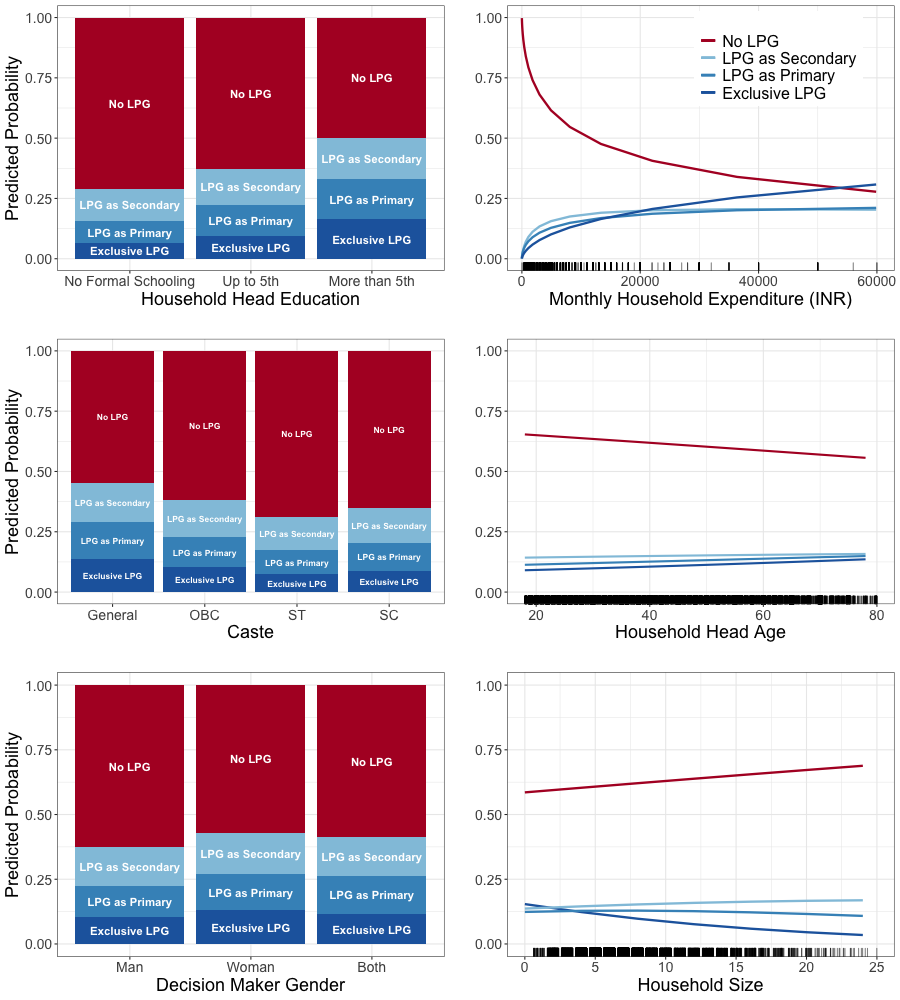
\includegraphics[scale=0.55]{Figures/Marginal_Effects/gologit_rugs.png}
\caption{\textbf{Predicted probability of fuel stacking category from generalized ordered logit model.} Figure shows the comparison of predicted probability (0-1) of four levels of LPG adoption: exclusive LPG use, LPG as primary, LPG as secondary, and no LPG use. The sum of the probabilities is equal to 1. Tick marks on the x-axis indicate all individual data points to show the distribution of each variable.}
\label{f:gologit_ME}
\end{figure}

Next, we jointly model LPG adoption and use. We present results from the double-hurdle model as the average-adjusted predicted probability of LPG adoption and then the amount of LPG consumed in kilograms (kg) each month (Fig. \ref{churdle_ME} and \textit{SI Appendix}, Table \ref{t:gologit&hurdle}). Average-adjusted predicted probabilities are those where all other covariates are held at their averages.

We find similarity between the predictors of LPG adoption and use. Households with greater wealth, more educated household heads, and those that belong to the general caste category have higher predicted probability of adopting LPG and consuming more LPG per month than their peers. 

The average-adjusted predicted probability of LPG adoption when the household head has attained an education more than 5th Standard  is 48.5 percentage points (95\% CI: 46.7-50.1 percentage points), a full 13.5-21.5 percentage points higher than households where the household head has attained a primary education or no formal education. After adoption, households with a household head attaining an education more than 5th Standard are predicted to consume -- holding all other covariates at their means including household size --  7.4 kg of LPG per month (95\% CI: 7.2-7.6 kg). In comparison, households with less formally education household heads are predicted to consume between 0.4 and 0.9 kg per month less. Over the course of a full year, then, households with household heads attaining more than 5th Standard education consume between one-half to two-thirds of a large 14.2 kg cylinder of LPG more than their counterparts.

Trends are similar for caste. Households belonging to the general caste have an average-adjusted predicted probability of owning LPG  7.3-15.2 percentage points higher than households belonging to the scheduled caste, scheduled tribe (indigenous communities), or other backward class (other communities that are recognized as socially disadvantaged). Then, a household in the general category is predicted to consume about one half of a large 14.2 kg cylinder of LPG more than their counterparts.

The relationships between increases in monthly expenditures and LPG adoption and use are highly non-linear for expenditures below 10,000 INR per month (approximately 85\% of households spend fewer than 10,000 INR per month), increasing rapidly at low expenditures and leveling off at higher expenditures. Each month, households at the 75th percentile (7,000 INR per month) of monthly expenditures are predicted to consume 0.6 kg of LPG more (7.2 kg per year more) than those at the 25th percentile (3,000 INR per month). In addition, while larger households have a lower predicted probability of adopting LPG, once adopted, larger households are predicted to consume more LPG than smaller households.

Perhaps most notably, however, we also find that PMUY beneficiaries consume significantly less LPG after adoption than their general customer counterparts. PMUY beneficiaries have an average-adjusted predicted probability of consuming 5.3 kg of LPG per month (95\% CI: 5.1-5.5 kg). In comparison, general customers are predicted to consume 7.6 kg per month (95\% CI: 7.4-7.7 kg). Accounting for all baseline differences -- including education, caste, monthly expenditures, household size, and years of owning LPG -- PMUY beneficiaries are predicted to consume 2.3 kg of LPG per month less (nearly two full large cylinder refills each year) than a household that acquired LPG independent of PMUY. 

We also find that households are predicted to consume LPG more the longer they have had the stove. After the first year of ownership, households are predicted to consume 6.6 kg of LPG per month (95\% CI: 6.4-6.7 kg). Holding all else constant, households with three more years of experience with LPG are predicted to consume 5 kg per year more than in year one.


\begin{figure}[h!]
	\centering
	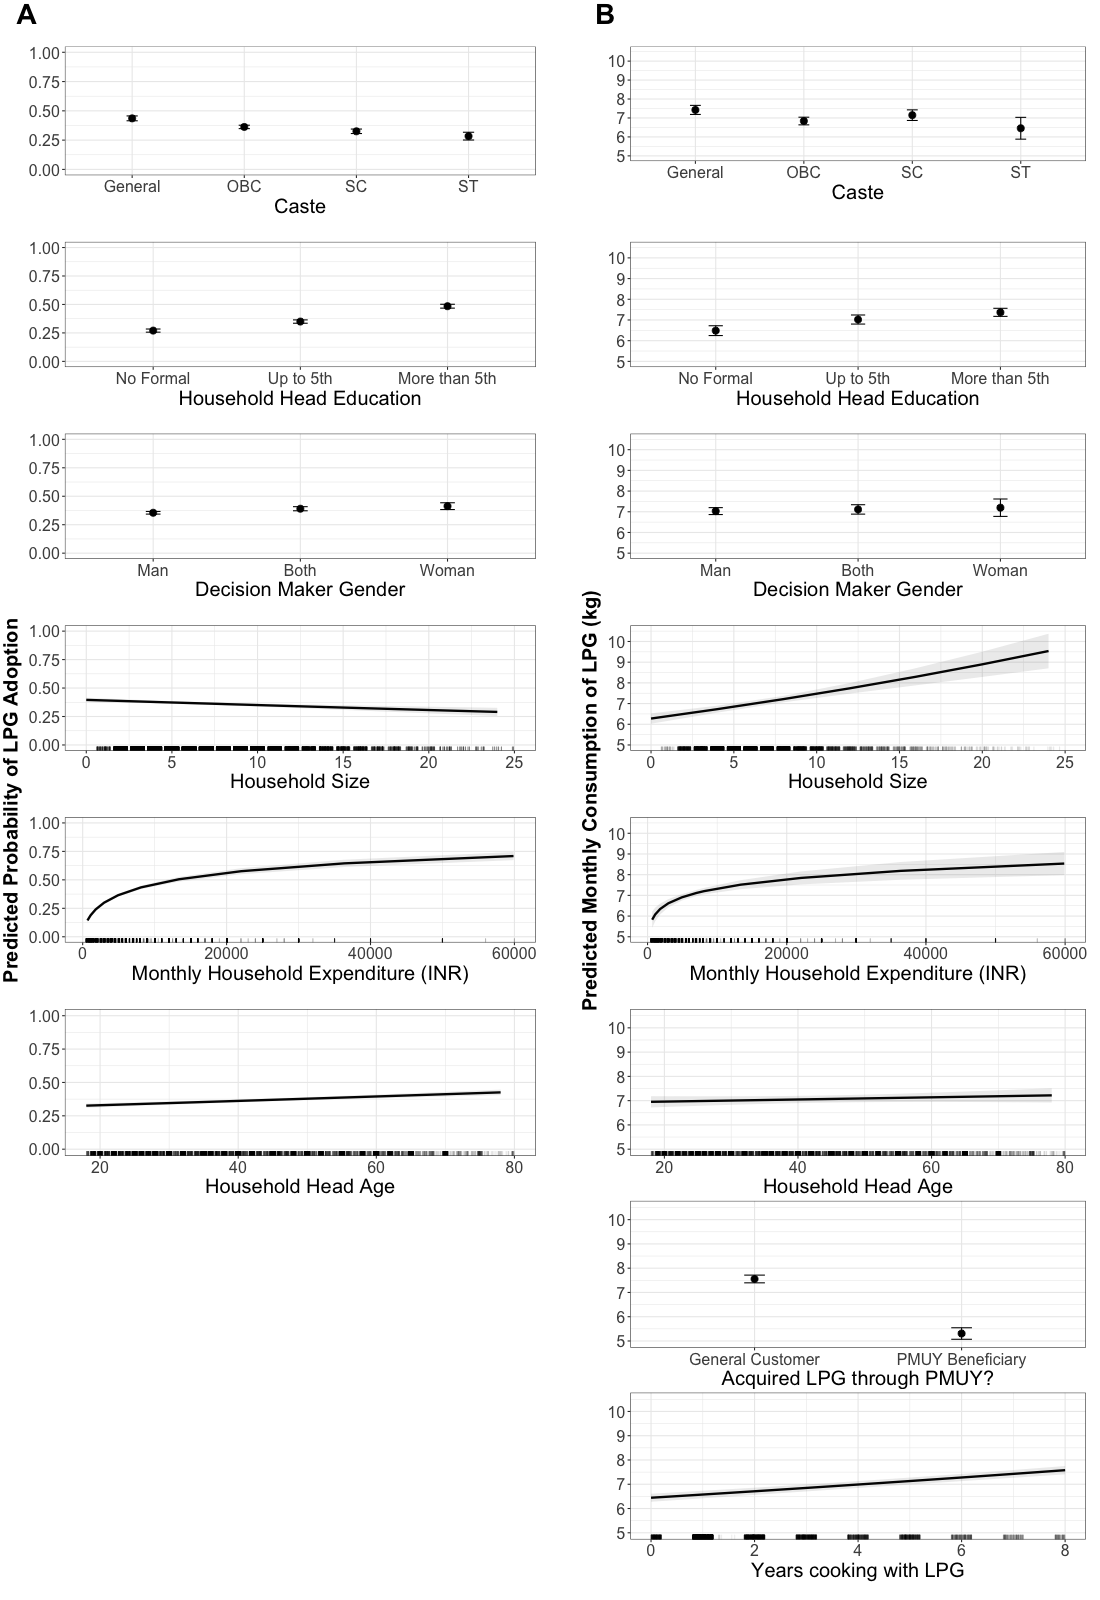
\includegraphics[scale=0.38]{Figures/Marginal_Effects/churdle_ME_option2_rugs.png}
	\caption{\textbf{Average adjusted predictions of LPG selection and consumption from two-stage double-hurdle model with 95\% confidence intervals.}  \textbf{A.} The left panel shows the average-adjusted predicted probability of LPG adoption between 0 and 1 in the model's first stage with 95\% confidence intervals. \textbf{B.} The right panel shows the average-adjusted prediction of monthly consumption -- on condition of LPG adoption -- in kilograms in the model's second stage. Standard errors in the both model stages are clustered by village. Tick marks on the x-axis indicate all individual data points to show the distribution of each variable.} 
	\label{churdle_ME}
\end{figure}

\textbf{Inclusion of Village-Level Covariates.} We find that our results are robust to accounting for additional village-level covariates. The coefficients presented in the main results for both the gologit model and the double-hurdle model do not substantively change in this alternative specification (\textit{SI}, Table \ref{t:gologit&hurdle_app_full} and Figs. \ref{gologit_village}, \ref{churdle_ME_village}). We find that the distance required to get an LPG cylinder refill is negatively associated with LPG adoption and use. In addition, distance to the nearest town is negatively associated with LPG adoption and use, with a more pronounced effect between 0 and 15 km that weakens at greater distances. Villages size is positively associated with LPG adoption, but only weakly associated with use after adoption. Still, larger villages tend to have more households that exclusively use LPG. Somewhat surprisingly, households in villages with greater forest cover have higher probabilities of adopting LPG and using it more after adoption. However, we do not interpret these results to mean that greater biomass availability leads to greater LPG adoption and use, but rather that perhaps nearby forest cover is associated with other determinants of cooking fuel use in ways we cannot capture.


\section*{Conclusion}

Expanding clean cooking is a priority issue in India. Exposure to household air pollution is responsible for approximately half a million premature deaths in India each year, and the use of solid fuels for cooking is the most important driver of the problem. Furthermore, recent efforts have shown that household emissions from cooking with solid fuels accounts for approximately 30\% (range of estimates: 22\%-52\%) of all ambient air pollution in India\citep{Chowdhuryetal2019a}. Together, household air pollution and ambient air pollution are the second largest risk factor for ill-health in India behind poor nutrition\citep{Dandonaetal2017}. Three-quarters of Indians are exposed to air quality levels above the Indian National Ambient Air Quality Standard\citep{Balakrishnanetal2019}. Yet, abating household solid fuel use can bring India's population-weighted average air pollution exposure to the National Ambient Standard, averting hundreds of thousands of premature mortalities each year\citep{Chowdhuryetal2019b}. In this study, we have explored India's nascent and ambitious transition away from solid fuels and toward LPG as a clean cooking fuel.

Using two panels of data collected in rural households across six north Indian states, we find that drivers of LPG adoption, LPG use, and exclusive use of LPG are similar. Most importantly, both household expenditure (a proxy for income) and education have large positive impacts on all three outcomes, accounting for both shifts toward cleaner cooking fuel stacks and overall LPG use. While the traditional ``energy ladder'' model\citep{Leach1992} fails to capture the logic of fuel stacking, our results show that in rural north India the transition from solid fuels to LPG is nonetheless quasi-linear in nature. Households first adopt LPG as they grow wealthier and more educated; they then drop solid fuels altogether as this progression continues. Variation in fuel stacking, then, is driven by the same factors that explain variation in the adoption of clean cooking fuels in the first place.

These results have important implications for the Government of India and other policymakers aiming to improve health through reductions in HAP exposure. One of the major challenges of such efforts has been that households adopt clean cooking fuels but engage in fuel stacking, i.e., households continue to use solid fuels, and fail to capitalize on the potentially sizable health benefits of clean cooking. Our results suggest, however, that the same factors that drive LPG adoption also encourage reduced reliance on solid fuels and eventually exclusive use of clean cooking fuels. While rural income and education are broad challenges that reach well beyond household energy, their importance does highlight affordability and awareness as potential interventions. 

In this regard, Government of India's PMUY scheme is a logical step forward. However, we find that PMUY beneficiaries consume nearly two large cylinders of LPG less than general customers, accounting for education, monthly expenditures, caste, household size, gender of the decision-maker, age of the household head, and years with LPG. These findings point to distinct differences between PMUY beneficiaries and general customers, beyond socio-economic differences and experience with LPG. While we find that households using LPG for longer do consume the fuel more, these increases are modest and would not be expected to yield full displacement of solid fuel use even after five years.

Given the magnitude of the negative effects of continued solid fuel use, additional actions are needed to accelerate the transition toward exclusive clean cooking fuel use. To address cost considerations, the Government of India may consider more targeted subsidies to poorer households and PMUY beneficiaries that currently have low cylinder refill rates. Indeed, the Government of India is actively considering subsidizing cheaper and smaller 5 kg LPG cylinders (the typical size is 14.2 kg) to address low cylinder refill rates. Our finding that households in villages with closer access to LPG cylinder refills consume more LPG after adoption suggests that increasing the number of local distributors may yield greater LPG consumption in rural areas.

Recent studies have explored several strategies to accelerate both the uptake and use of clean cooking fuels in rural India, including: lowering stove costs\citep{Pattanayaketal2019,Menghwanietal2019}, lower fuel costs or free fuel\citep{Pillarisettietal2019}, improved fuel accessibility\citep{Pattanayaketal2019,Pillarisettietal2019}, and providing a second LPG cylinder to reduce gaps in fuel\citep{Pillarisettietal2019}. With respect to addressing awareness, future programs may include education on the benefits of clean cooking and capacity training on the use and safe handling of LPG stoves and cylinders to increase use. A recent effort in India suggests that health messaging as a part of a package of a clean cooking intervention accounting for other supply-side issues may discourage solid fuel use\citep{Pillarisettietal2019}. Importantly, health messages as an intervention in isolation have not been effective at changing cooking habits\citep{Shankaretal2014}. 

Integrated policies and programs that comprehensively address the issues that limit clean cooking can yield large social and health benefits for hundreds of millions of Indians. There is no one solution to achieving exclusive clean cooking fuel use in rural Indian households. Future efforts will need to respond to local contexts, the multiple constraints of poor and rural households, and preferences for household energy technologies -- including non-cooking end uses like heating. However, combinations of awareness campaigning and measures to enhance the affordability and accessibility of clean cooking fuels can help hundreds of millions in rural India lead healthier and more productive lives. 


\clearpage

\section*{Methods}

Here, we summarize the study sampling design and data used, our choices for dependent and independent variables, and statistical approaches for assessing the determinants of household cooking fuel choices. 

\subsection*{Two-wave representative survey of energy access in north India}

We use the Access to Clean Cooking Energy and Electricity -- Survey of States (ACCESS), a two-wave panel dataset\citep{Manietal2018}. Briefly, the sampling frame included 714 villages across 51 districts within the north Indian states of Bihar, Jharkhand, Madhya Pradesh, Odisha, Uttar Pradesh, and West Bengal. These north Indian states were selected because they have historically been energy poor; furthermore, they combine to account for 500 million individuals or almost 40\% of the country's population. In 2015, sampling was done using a three-stage probability-proportional-to-size (PPS) survey design. Previously, the ACCESS study team has shown that the sampling design has yielded a representative sample as compared to the 2010 National Sample Survey\citep{Aklinetal2016}. Nonetheless, sampling weights are used throughout to account for variations in district household populations. We describe the sampling design and survey implementation further in the Supplementary Information. 

A household energy access and use survey was administered to 8,563 households in the first wave of the survey collected between November 2014 and May 2015 and 9,072 households in the second wave collected between April 2018 and September 2018. If the household head in a household surveyed in 2015 was unavailable, enumerators interviewed any other willing adult in the household. If no adult was available or willing to participate then the household was replaced with the fifth household walking to the right of the original household. In total, the attrition rate between waves was 14\% (\textit{SI Appendix}, Table \ref{t:retention}) and was accounted for with the aforementioned replacement sampling. In the second wave, additional households were sampled in three new districts of Odisha to balance sample sizes across study states. 

In total, the ACCESS dataset includes household energy data from 17,640 households across both waves. While the general survey was directed to the household head or other willing adult, primary cooks were interviewed and/or present for the cooking modules used in the present study.


\subsection*{Dependent variables}

We use three outcome variables to describe cooking fuel choice. First, the outcome variable for the gologit model is an ordinal discrete choice variable with four ordered categories: 1) no LPG and firewood or other solid fuel used for cooking, 2) fuel stacking with LPG as a secondary cooking fuel and firewood or other solid fuel as the primary cooking fuel, 3) fuel stacking with LPG as the primary cooking fuel and firewood or other solid fuel as a secondary cooking fuel, and 4) exclusive LPG use. Second, we utilize a two-stage variable in the double-hurdle model. The first-stage outcome is a binary variable for LPG ownership (0 = No LPG and 1 = Owns LPG). The second-stage outcome variable is a continuous variable for the amount of consumption of LPG among adopters or those who participate in the market. We specify LPG consumption in kilograms per month, computed from self-reported LPG cylinder refills purchased in the past year multiplied by 14.2 kg (the typical cylinder size in India) and divided by 12 months. 

\textit{SI Appendix} Tables \ref{t:sum_dependent_2015} and \ref{t:sum_dependent_2018} outline the distribution of fuel stacking categories in 2015 and in 2018, respectively. \textit{SI Appendix} Fig. \ref{bar_fuel_stack} does so graphically. \textit{SI Appendix} Fig. \ref{distribution_lpg_log} shows the distribution of LPG consumption among study participants in kilograms per year.

\subsection*{Independent and control variables}
\label{sect:variable_specification}

We identified covariates for inclusion in our models from previous studies of the determinants of clean cooking fuel adoption and use, drawing in particular on several reviews\citep{MullerYan2018,Puzzoloetal2016,LewisPattanayak2012}. Given the computational demands of the two-stage double-hurdle model, we aimed to achieve a parsimonious model that adequately accounts for potential omitted variable bias. Here, we briefly explain our choices for covariates. \textit{SI Appendix} Tables \ref{t:sum_indep_2015} and \ref{t:sum_indep_2018} summarize the distributions of independent variables in 2015 and in 2018, respectively.

\textit{Monthly expenditure} is a common explanatory variable in studies of clean cooking adoption and use\citep{MullerYan2018}. Broadly, monthly expenditures are applied in this context as estimates of household material well-being, a common and effective practice in circumstances where measured incomes may be rare on unreliable\citep{Klasen2000}. Increased wealth and well-being are positively associated with increased clean cooking fuel adoption and use\citep{LewisPattanayak2012}. In addition, there have  been several studies specifically linking expenditures to clean cooking fuel adoption and use (including LPG) \citep{SaxenaBhattacharya2018,Heltberg2004,GuptaKohlin2006,Farsietal2007}.

\textit{Household size} may play a role in cooking fuel choice through different avenues. For instance, larger households may demand more cooking in terms of frequency and quantity, therefore necessitating multiple cookstoves, more cooking, or more efficient cooking depending on other priorities. In addition, households with more adults are likely to have different levels of income and expenditure, which could directly affect LPG adoption and use. However, household size has had different directions of association in empirical studies. Some have shown that larger households are more likely to cook with solid fuels\citep{RaoReddy2007,PandeyChaubal2011}, while others have shown that larger households are more likely to use a clean cooking fuel\citep{GuptaKohlin2006,BaiyegunhiHassan2014}. Elsewhere there has been no statistically significant association\citep{Chenetal2006}. Additionally, Heltberg (2004) (ref. \cite{Heltberg2004}) find that larger households are more likely to stack multiple fuels, but household size does not necessarily explain the exclusive use of any fuel. 

\textit{Education of the head of household} is emphasized in studies of the determinants of cleaner cooking\citep{MullerYan2018} as well as in the broader environmental health intervention literature\citep{Dreibelbisetal2013}. Education may serve as an indicator of awareness of clean cooking, knowledge of the burdens of traditional cooking practices, ability to obtain alternative fuels, greater household wealth, greater opportunity cost for solid fuel collection, or a different willingness to pay for alternative fuels. Previously, increased education has been associated with clean cooking fuel adoption and use\citep{Dalabaetal2018,Wolfetal2017} as well as reduced use of solid fuels\citep{Abebaw2008}. In this study, we specify education of the household head as a categorical variable: 1) no formal schooling (the baseline), 2) up to 5th standard, and 3) greater than 5th standard. 

\textit{Government-scheduled caste or tribe} has been shown to be associated with lower overall socio-economic outcomes in India due to long-standing marginalization and social exclusion\citep{DesaiDubey2012}. Studies of cooking fuel choice in India often included caste, finding a negative association with cleaner cooking\citep{Menghwanietal2019,SaxenaBhattacharya2018,Kumar2017,LewisPattanayak2012}. We specify caste in four categories: 1) general category (the baseline), 2) scheduled caste, 3) scheduled tribe (indigenous communities), or 4) other backward class (an official term for other historically educationally and socially disadvantaged groups).

\textit{Women's participation in decision-making} and gender, generally, is a debated aspect of household cooking fuel choice. Given that women generally bear primary cooking responsibilities, their involvement in decision-making may explain fuel choice based on specific cooking fuel preferences, such as lack of smoke, speed, ability to cook more of food, ability to cook all types of food, and familiarity. A growing body of literature supports a positive association between women-headed households and the use of clean cooking fuels\cite{Kumar2017,Beheraetal2015,Rahutetal2014,Heltberg2004}. However, few directly model women's involvement in decision-making\citep{Menghwanietal2019}. In this study, participants were asked, ``Who in your household makes decisions on the purchase of durable goods?" Responses were categorized as 1) man, 2) woman, or 3) both man and woman. Using data from the first wave of ACCESS, we establish a robust positive association between women decision-makers and LPG adoption\citep{GouldUrpelainen2019}. 

\textit{Religion} can serve as an indicator of class welfare that can be linked to fuel choice. In rural India, followers of Hindu religions are the dominant majority, while Buddhists, Muslims, and Christians are often minorities that may exhibit lower overall socio-economic outcomes because of their marginalized position in society\citep{BorooahIyer2005}. Identifying as Muslim, in particular, has been shown as a significant indicator of social inequality\citep{SaxenaBhattacharya2018}. Previous studies of cooking fuel choice in India have included religion\citep{Menghwanietal2019,Bhojvaidetal2014,LewisPattanayak2012}. Here, the baseline category is a combination of religions other than Hindu.

\textit{Age of the household head} may affect cooking fuel choice, and is commonly included in empirical studies of cooking fuel choice. However, there have been contradictory results to date\citep{MullerYan2018,LewisPattanayak2012}, with some studies showing that households with older households heads are more likely to use solid fuels\citep{BaiyegunhiHassan2014}, clean cooking fuels\citep{Wolfetal2017,Farsietal2007,GuptaKohlin2006}, or even no association\citep{Menghwanietal2019,Abebaw2008}. 

\textit{PMUY beneficiaries} have been show to consume less LPG than general customers in previous studies\citep{Karetal2019b,Tripathietal2020}, and in government databases on cylinder refills\citep{CAG2019}. Understanding LPG consumption patterns after adoption through PMUY is one of the policy's most pressing questions, and a key to yielding the full benefits of LPG adoption for tens of millions of Indian households.

\textit{Years of LPG experience} may affect consumption or use of LPG and other cooking fuels in the household for a variety of reasons. For example, households that have used LPG longer may have increased familiarity and ability with the cooking style. In addition, it is possible that cooking with LPG for longer has yielded shifts in attitudes and preferences towards LPG cooking or traditional cooking styles. Years of cooking with LPG has been positively associated with LPG consumption elsewhere\citep{Dickinsonetal2019,Dalabaetal2018,Tripathietal2020}.

In an additional analysis we include four unique village-level covariates. Together, these covariates serve as proxies for LPG fuel accessibility. It is relevant to note that there is little variation in LPG cylinder costs across this region of India because prices are set by state-run oil companies and only revised on a monthly basis, as well as robust cylinder subsidies.

\textit{Number of households in the village} accounts for the robustness of LPG cylinder supply. Households living in urban communities consistently use more clean cooking fuels and less solid fuels for cooking than their rural counterparts. Improved socio-economic development often accompanies the growth in community sizes, which leads to improved infrastructure and increased reliability of clean fuel supply\citep{RaoReddy2007}. We calculate village size using data from the 2011 National Census (for all villages except those in West Bengal) and 2001 National Census (for villages in West Bengal). In the ACCESS project we estimated the number of households in a village by speaking to a village leader. However, 232 villages had missing data, which would lead to 5,313 dropped households. We utilized Census data to avoid losing this quantity of data. Given the across-village nature of our analysis, we expect that the proportional differences between villages is more important than employing more current data. 

\textit{Distance to the nearest town} is a proxy for LPG cylinder supply. Previously, distance to the nearest town has been used to predict solar electrification in India\citep{Aklinetal2018}. We follow methods previously established by study collaborators (ref. \citep{Aklinetal2018}) and use 2011 National Census data to estimate the straight line distance (in kilometers) from village centers to the nearest statutory town, or an urban area with a municipal corporation or equivalent governing body.

\textit{Average one-way distance traveled to acquire an LPG cylinder refill} is a direct self-reported measure of the burden of LPG cylinder acquisition. LPG-owning respondents were asked ``What is the one-way distance in kilometers your family typically travels to get LPG?" We averaged all responses within a village to estimate the covariate. Long travel distances may be a limiting factor in transitions away from reliance on solid fuels to clean cooking fuels\citep{Houetal2017}.

\textit{Forest cover} is used here as an indicator for biomass availability. Previous studies have pointed to biomass availability as a driver of cooking fuel choice\citep{Beheraetal2015,JaggerKittner2017,JaggerShively2014}. Using freely-available information from The Socio-Economic High-resolution Rural-Urban Geographic Dataset on India (SHRUG v1.2)\citep{Asheretal2019}, we identify forest cover in 2014 from the vegetation Continuous Fields 250 meter resolution data for each study village. These data provide annual tree cover in the form of each pixel under forest cover based on multiple MODIS images and additional higher-resolution satellites as used previously\citep{Asheretal2018}. For our variable of interest, we define average forest cover for each study village as total forest cover in the provided village polygons (based on the 2011 Census) divided by the total number of pixels comprising each polygon. Therefore, average forest cover provides us with a percentage of the total area associated with each village labeled as forest. 

\subsection*{Statistical Approach}

The primary goal of this study is to model the determinants of cooking fuel choice. We evaluate the household decision process to first adopt and then use LPG for cooking. To do so, we first use a generalized ordered logit (gologit) model to assess the determinants of fuel choice, categorized into four fuel stacks: exclusive solid fuel use and no LPG, solid fuel as the primary cooking fuel with LPG as a secondary cooking fuel, LPG as a primary cooking fuel with continued use of solid fuel as a secondary option, and exclusive LPG use. Second, we use a two-stage double-hurdle model to jointly assess the determinants of the decision to adopt LPG and then the expected amount of LPG consumption among adopters.

\subsection*{Generalized Ordered Logistic Regressions}

To address our research question of what determines a household's decision to stack fuels and how households decide to prioritize stacked fuels, we use a generalized ordered logistic regression (gologit) model. The gologit model is presented in its formal notation in the Supporting Information. We order our fuel stacking categories from most reliant on LPG to least reliant on LPG (1 = exclusive LPG use, 2 = LPG as a primary cooking fuel but maintains the use of a solid fuel for cooking, 3 = solid fuel as the primary cooking fuel but uses LPG as supplementary cooking fuel, 4 = exclusive solid fuel use). Since our outcome variable for fuel stacking is an ordinal variable, we have chosen an appropriate ordered discrete choice model. As Williams (2006) (ref. \citep{Williams2006}) discusses, a gologit model is typically used to correct for a violation of the parallel lines assumption found when running an ordered logistic regression (ologit). The parallel lines assumption is that all of the estimated $\beta$s for explanatory variables are statistically the same value for each category of the outcome variable; only the intercept would change significantly, allowing for an interpretation that estimates the difference between parallel lines.

In our case, however, the parallel lines assumption is violated in the ologit model by a subset of variables. As carried out elsewhere (ref. \citep{Williams2006}), we use a Brant test to parse out each binary regression between categories of our dependent variable. To illustrate, our outcome variable has four categories: 1) firewood or other biomass only, 2) fuel stacking with LPG as a primary source, 3) fuel stacking with other fuel sources as a primary source, and 4) exclusive LPG use. Therefore, when we run the Brant test, we collapse our categories in each of three binary regressions that are required to test for the probability that $y>1$, $y>1,2$, and $y>1,2,3$. We find that the test is significant at $\alpha = 0.05$, suggesting that we would overestimate or underestimate the marginal effect of moving away from each category or group of categories if we relied on the ologit model with strict assumptions. According to our test results, the constraints for parallel lines are not imposed for the following variables: monthly expenditure, household size, gender of the decision maker (category: both man and women are joint decision-makers), religion (Hindu), indicator variables for certain states (Bihar, West Bengal, Jharkhand, and Madhya Pradesh), and the indicator variable for survey wave.

Therefore we choose the gologit model to relax the parallel lines assumption. The gologit model offers a straightforward interpretation of partial proportional odds for each comparative outcome between our categories (again, $y>1$, $y>1,2$, and $y>1,2,3$). In comparison to the ologit model, the gologit model estimates different coefficients for each of the binary regressions between these collapsed categories to provide a more accurate estimate of movement from one category to the next (rather than the same coefficient for different intercepts). The vector of parameters is estimated through maximum likelihood estimation.

We use a user-written program in Stata to fit a partial proportional odds model for fuel stacking\citep{Williams2006}. We present results as predicted probabilities (referred to as predictive margins in Stata) calculated for hypothetical cases using the ``margins" command\citep{Williams2012}. We use the ``at()" option to fix the variable of interest at a specific value, which facilitates the comparison of predicted probabilities between different categories by providing a simple comparison of the relative influences of covariates. We present average marginal effects (AMEs) instead of marginal effects at the means (MEMs) to use actual observed values for unfixed variables instead of using their means. With this method, we calculate the probabilities of each case and then average the predicted values to represent the average probabilities of different fuel stacking under the fixed variable. We can then compare two hypothetical population groups that have the exact same values for other unfixed covariates and only different in the variable of interest.

\subsection*{Hurdle Models}

Next, we jointly model the determinants of LPG adoption and the predicted amount of LPG consumption using a two-stage double-hurdle model. This model, originally formulated by Cragg (1971)
(ref. \cite{Cragg1971}), assumes a decision to consume a good is made in two stages. First, participants decide to participate (here, to adopt LPG). Second, consumers decide their optimal consumption (here, how much LPG to use per month in kilograms)\cite{Garcia2013}. It is plausible that the determinants of the decision to participate and the determinants of consumption are different and, therefore, a two-stage double-hurdle model is ideal for jointly modeling LPG adoption and use. 

In our formulation, we test the same set of covariates in both steps of the two-stage double-hurdle model (also the same as those utilized in the gologit model and described in Section \ref{sect:variable_specification}). We use the ``churdle" command in Stata and define that the outcome variable is truncated at 0. We then calculate average-adjusted probabilities for participation (LPG adoption) in stage 1 and average-adjusted predicted LPG consumption (LPG use) in stage 2 using margins command.

The double-hurdle model estimates four equations in two distinct stages. The first equation estimates the decision to adopt LPG in a binary logit model. This step is the ``hurdle" that households need to overcome to use LPG. Then, the second equation models the expected amount of consumption for those who participate in the LPG market. This model uses a truncated Poisson model to estimate LPG consumption in kilograms. Third, the standard deviation of the error term in the first equation is estimated. The fourth equation then estimates covariance between the error terms of the first two equations for the decision to adopt LPG and then how much LPG is consumed.

A double-hurdle model may be more ideal than tobit models when dealing with corner solutions (individuals with no option to participate in the LPG market or who refuse to participate no matter the circumstances)\cite{Garcia2013}. When the decision to adopt a technology is distinct from the decision to use it, as is the case here, a double-hurdle model offers an appealing alternative to isolate the expected probability of the amount of consumption among those who have chosen to participate in the market. 

\subsection*{Ethical Considerations}

The study protocol was reviewed and approved by the Johns Hopkins University Institutional Review Board and [*** XXXXXX ***]. Informed consent was obtained from all study households.

\subsection*{Data Availability}

The data and code used in this study are available at [** XXXX **].

\clearpage

\bibliographystyle{naturemag}
\bibliography{../cooking}

\end{document}